\documentclass[12pt, letterpaper]{article}
\usepackage{graphicx} % Required for inserting images
\usepackage{hyperref}
\usepackage{listings}
\usepackage{amssymb}
\usepackage{amsmath}
\usepackage[english]{babel}
\usepackage{nicefrac, xfrac}
\usepackage{mathtools}
\usepackage[utf8]{inputenc}
\newcommand{\acc}{\\\hphantom{}\\}
\usepackage[dvipsnames]{xcolor}
\usepackage[table,xcdraw]{xcolor}
\definecolor{light-gray}{gray}{0.95}
\newcommand{\code}[1]{\colorbox{light-gray}{\texttt{#1}}}
\newcommand{\codee}[1]{\colorbox{white}{\texttt{#1}}}
\usepackage[paper=a4paper,left=20mm,right=20mm,bottom=25mm,top=25mm]{geometry}
\renewcommand{\labelenumii}{\arabic{enumi}.\arabic{enumii}}
\renewcommand{\labelenumiii}{\arabic{enumi}.\arabic{enumii}.\arabic{enumiii}}
\renewcommand{\labelenumiv}{\arabic{enumi}.\arabic{enumii}.\arabic{enumiii}.\arabic{enumiv}}
\newcommand{\id}{{\hphantom{ident}}}
\newcommand{\vincolo}[1]{\colorbox{Orange}{$[$\text{#1}$]$}}
\title{\textbf{TuTubi}}

\date{}


\begin{document}

\maketitle
\section{Specifica delle Classi}
\subsection{Classe Video}
\subsubsection*{Operazioni}

\begin{verbatim}
durataSec() : Intero >= 0
    pre: nessuna
    post: 
        result = durataSec(this.flusso)

n_visualizzazioni() : Intero >= 0
    pre: nessuna
    post:
        result è il numero di oggetti v:Visualizzazione tali che:
            (this, v): vid_vis

valutazioneMedia() : float >= 0
    pre: nessuna
    post:
        sia valutazioniVideo un insieme che contiene tutti gli oggetti 
        di tipo Visualizzazione per cui esiste un link (this,visualizzazione): vid_vis
        sia vTot la somma di tutti i visualizzazione.valutazione in valutazioniVideo
        return vTot / |valutazioneVideo|

num_risposte() : int >= 0
    pre: nessuna
    post: 
        sia insiemeRisposte un insieme contentente tutti gli oggetti 
        di tipo Video per cui esiste un link (v,Video): risposta_a_video
        ritorna |insiemeRisposte|
\end{verbatim}
\subsection{Attenzione}
Tutte le altre classi, poichè prive di operazioni sono state omesse per semplictità.
\newpage\section{Specifica Tipi di Dato}

\textbf{FileVideo}: 
\begin{verbatim}
 - sequenza di byte che codifica un flusso video
 - operazioni del tipo di dato
 		durataSec(f:FileVideo): Intero >= 0
 			pre: nessuna
 			post: result è la durata di 'f'
\end{verbatim}
\section{Specifica dei vincoli esterni}
\vincolo{V.Video.autore\_non\_risponde\_a\_se\_stesso} \\
Per ogni r:Video, per cui esiste v:Video tale che\\
\id(r,v): risponde\_a\_video\\
\id sia:\\
\id\id- u:Utente tale che:\\
\id\id (u, r): pubblica\\
\id Deve che (u,v) non è un link di pubblica.\\
\id Formalmente:\\
	$$ \begin{matrix}\forall r,v,u \;\;\;  Video(r) \land Video(v) \land Utente(u) \land \\
				pubblica(u,r) \land \\
				risponde\_a\_video(r,v)  \;\;\;\rightarrow\\
                \lnot pubblica(u,v) \end{matrix}$$
\vincolo{V.Visualizzazione.valutare\_proprio\_video} \\ 
Per ogni utente $u$, sia $VIS$ l'insieme degli oggetti di tipo $Visualizzazione$ 
tale che:\begin{itemize}
    \item $\exists (u,vis):ut\_vis$ con $vis\in VIS$
    \item $\exists (vis,v):vid\_vis$ con $vis\in VIS$
    \item $\exists(u,v):utente\_pubblica\_video$
\end{itemize}
Deve essere che $\forall\; vis \in Vis,\;\;\;vis.valutazione=NULL$\\ 
\id Formalmente 
$$\begin{matrix} \forall u,\;v\;,vis\;\;Utente(u)\land Video(v)\land Visualizzazione(vis)\\
    \land ut\_vis(u,vis)\land vid\_vis(vis,v)\\\land utente\_pubblica\_video(u,v)\rightarrow \\ 
    valutazione(vis,NULL) 
\end{matrix}$$
\vincolo{V.Playlist\_no\_visualizza\_privata} \\ 
Per ogni utente $u$, se esiste $(u,p):puo\_visualizzare$ e non esiste $(u,p):crea$, 
allora deve essere che $p.pubblica=True$\acc
\vincolo{V.Video\_censurati} \\
Solo i video non censurati possono essere visualizzati, commentati, valutati o aggiunti a playlist.\\
\id Formalmente $$\begin{matrix}
    \forall v,\;vis,\;e\;\;\;Video(v)\land Visualizzazione(vis)\land Elemento(e) elem\_video(v,e)\lor vid\_vis(vis,v) \rightarrow \\ 
    censura(v,False)
\end{matrix} $$
\newpage

\section{Specifica Use Case}
\subsection{Registrazione}
\code{registrazione(n: Stringa): Utente}
\begin{itemize}
\item \textbf{Attori}: this, Utente Non Regirato
\item \textbf{Pre Condizioni}: Nessuna.
\item \textbf{Post Condizioni}: Viene Creata una nuovo oggetto di Classe Utente con:\\ Utente.nome =n (UNIVOCO)
e Utente.iscrizione = now.
\end{itemize}
\subsection{Pubblicazione Video}
\code{pubblicazioneVideo(t:Stringa, d: Stringa, f: FileVideo, c: Stringa, tag: Stringa): video}
\begin{itemize}
    \item \textbf{Attori}: Utente Registrato
    \item \textbf{Pre Condizioni}: Nessuna
    \item \textbf{Post Condizioni}: Viene creato un nuovo oggetto v di Classe Video con:
    \begin{itemize}
        \item v.titolo= t
        \item v.descrizione= d
        \item v.flusso= f
        \item v.istante=now
        \end{itemize}
    viene creato un link $(this, video): utente\_pubblica\_video$\\
    viene creato un link $(video, categoria): cat\_video$ con la categoria c del video\\
    vengono creati tanti link $(video, tag): tag\_video$ quanti sono i tag del video
\end{itemize}
\subsection{Cronologia}
\code{cronologia(): insieme videoVisualizzati}
\begin{itemize}
    \item \textbf{Attori}: Utente Registrato
    \item \textbf{Pre Condizioni}: Nessuna
    \item \textbf{Post Condizioni}: Viene restituito un insieme videoVisualizzati contentente tutti i video per cui esiste un link $(this,visualizzazione): ut\_vis$ e $(visualizzazione,video):vid\_vis$
    \\Tutti i video v per cui v.Censurato=True sono \textbf{esclusi} dalla cronologia.
\end{itemize}
\subsection{Ricerca}
\code{ricerca(c: Stringa, t:Stringa[0..*],v:int 0..5): video[0..*]}
\begin{itemize}
    \item \textbf{Attori}: Utente Registrato
    \item \textbf{Pre Condizioni}: Nessuna
    \item \textbf{Post Condizioni}: Viene restituito un insieme video[0..*] contentente tutti i video per cui esiste un link $(video, categoria): cat\_video$ con categoria c e per cui esiste un link $(video, tag): tag\_video$ con tag t[i] per ogni i=0..* e per $video.valutazioneMedia() >=v$.
    \\Tutti i video v per cui v.Censurato=True sono \textbf{esclusi} dalla ricerca.
\end{itemize}
\subsection{Ricerca Discussione} 
\code{ricercaDscussione(c: Stringa, t:Stringa[0..*],v:int 0..5): video[0..*]}
\begin{itemize}
    \item \textbf{Attori}: Utente Registrato
    \item \textbf{Pre Condizioni}: Nessuna
    \item \textbf{Post Condizioni}: Viene restituito un insieme video[0..*] contentente tutti i video per cui esiste un link $(video, categoria): cat\_video$ con categoria c e per cui esiste un link $(video, tag): tag\_video$ con tag t[i] per ogni i=0..* e per $video.valutazioneMedia() >=v$
    ordinati per $video.num\_risposte()$ decrescente.
    \\Tutti i video v per cui v.Censurato=True sono \textbf{esclusi} dalla ricerca.
\end{itemize}
\subsection{Gestione Playlist}
\code{creaPlaylist(n: Stringa, p: Bool): Playlist}
\begin{itemize}
    \item \textbf{Attori}: Utente Registrato
    \item \textbf{Pre Condizioni}: Nessuna
    \item \textbf{Post Condizioni}: Viene creato un nuovo oggetto di Classe Playlist con: Playlist.nome=n, Playlist.pubblica=p e Playlist.Data Creazione= now.
\end{itemize}
\code{aggiungiVideoPlaylist(p: Playlist, v: Video)}
\begin{itemize}
    \item \textbf{Attori}: Utente Registrato
    \item \textbf{Pre Condizioni}: v.Censurato=False.
    \item \textbf{Post Condizioni}: \\Viene creato un link $(p, elem): playlist\_elem$ con p playlist e elem un oggetto di tipo ElementoPlaylist con elem.NumeroVid un intero, tale intero è uguale al numero dei link $(p, elem): playlist\_elem +1$.
    \\Viene inoltre creato un link $(elem,v): elem_vid$ con v un oggetto di tipo Video.
\end{itemize}
\code{rimuoviVideoPlaylist(p: Playlist, v: Video)}
\begin{itemize}
    \item \textbf{Attori}: Utente Registrato
    \item \textbf{Pre Condizioni}: Esiste l'oggeto p di tipo Playlist video creato da this(Utente Registrato che invoca l'UseCase)
    \item \textbf{Post Condizioni}: \\
    Viene eliminato il link $(p, elem): playlist\_elem$ con p playlist e elem un oggetto di tipo ElementoPlaylist e aggiornati tutti i successivi video della playlist sottraendo un numero da ElementoPlaylist.NumeroVid.
    \\Viene inoltre eliminato il link $(elem,v): elem_vid$ con v un oggetto di tipo Video.
\end{itemize}
\subsection{Gestione Valutazioni}
\code{valuta(v: Video, val: int, c: Stringa): Valutazione}
\begin{itemize}
    \item \textbf{Attori}: Utente Registrato
    \item \textbf{Pre Condizioni}: this ha visualizzato il video v e v.Censurato=False.
    \item \textbf{Post Condizioni}: Viene creato un nuovo oggetto Valutazione di Classe Valutazione con: Valutazione.valutazione=val e Valutazione.istante=now.\\
    Viene creato un link $(this, valutazione): ut\_vis$ con this Utente Registrato.\\
    Viene creato un link $(valutazione, video): vid\_val$ con v Video.\\
    Viene creato un link $(valutazione, commento): val\_commento$ Commento.commento=c e Commento.Istante = now.
\end{itemize}
\subsection{Censura}
\code{censura(v: Video,m : Stringa)}
\begin{itemize} 
    \item \textbf{Attori}: Redazione
    \item \textbf{Pre Condizioni}: Nessuna
    \item \textbf{Post Condizioni}: Sia v un oggetto di classe Video.\\
    Viene impostato v.Censurato = true e v.MotivoCensura = m.\\
    Viene eliminato l'oggetto v da tutte le Playlist in cui è presente.\\
    Viene eliminato l'oggetto v da tutte le Cronologie degli Utenti.\\
\end{itemize}\newpage
\section{Diagrammi}
\subsection{Diagramma UML}
\begin{center}
    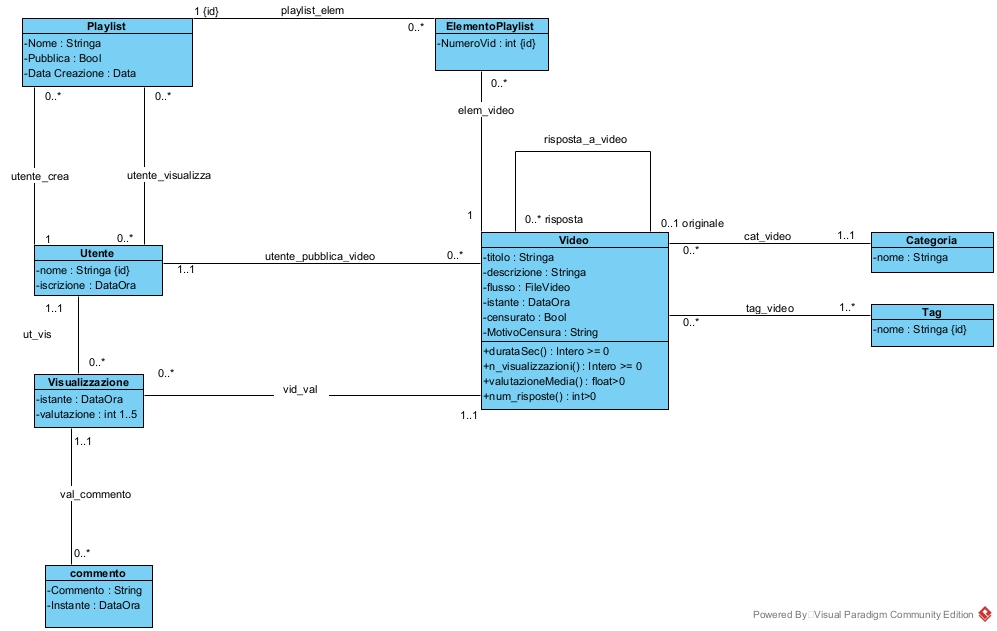
\includegraphics[width=1.1\textwidth ]{UML.jpg}
\end{center}\newpage
\subsection{Use Case}
\begin{center}
    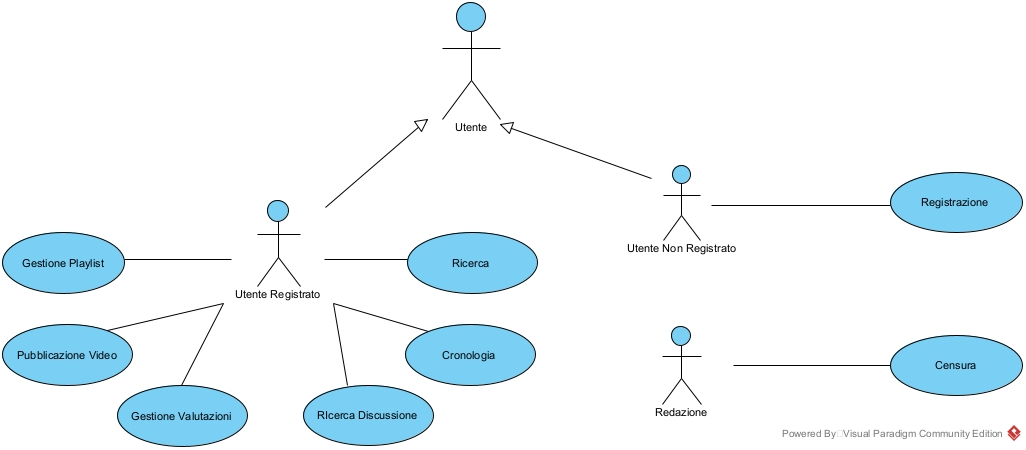
\includegraphics[width=1.1\textwidth ]{UseCase.jpg}
\end{center}
\end{document}